\section{Discussion}
\label{app:full_discussion}
\subsection{Limitations, failure cases and opportunities}
\label{sec:limitations}

\begin{figure}
    \centering
    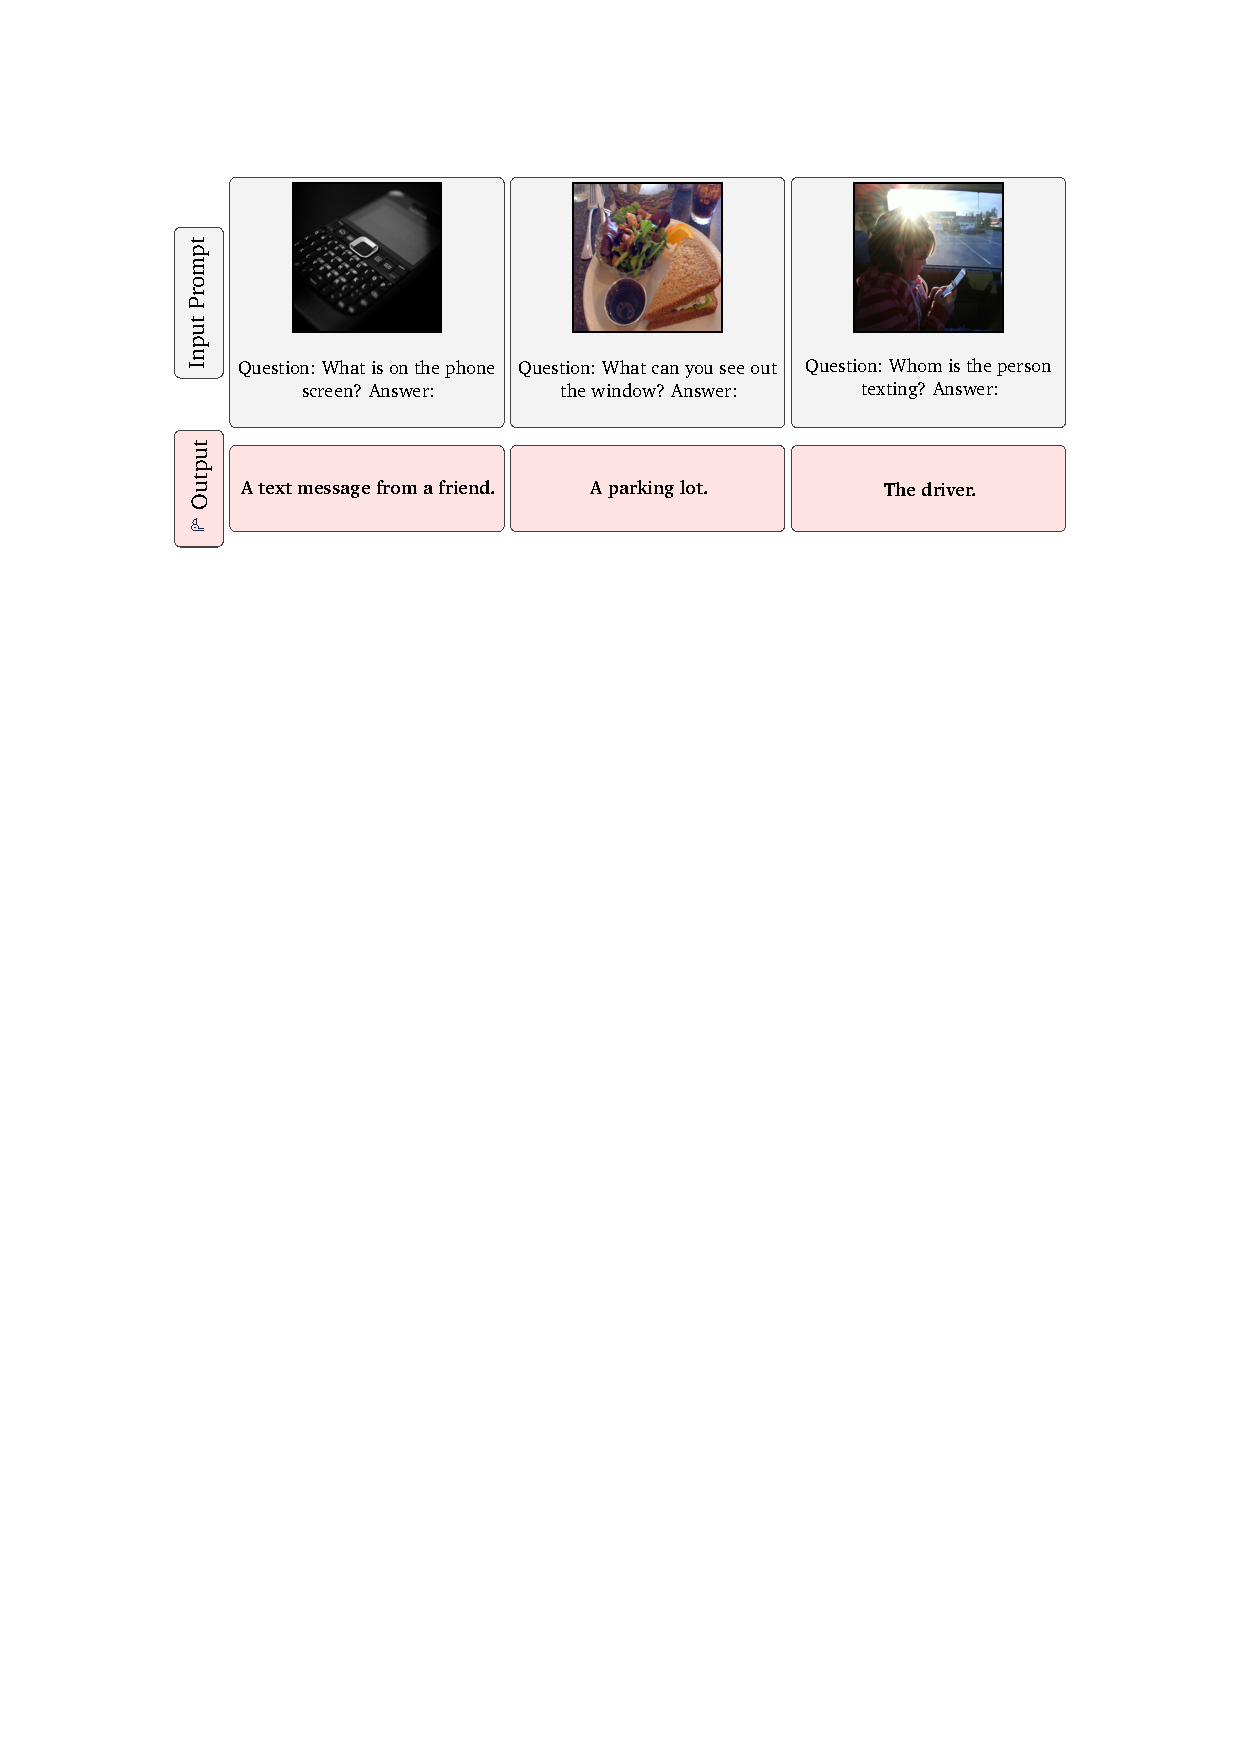
\includegraphics[width=\textwidth]{figures/failure_cases.pdf}
    \caption{
    \capfontsize{} \textbf{Hallucinations and ungrounded guesses in open-ended visual question answering.} %
    \textit{Left:} The model occasionally hallucinates by producing answers that seem likely given the text only, but are wrong given the image as additional input.
    \textit{Middle:}
    Similar hallucinations can be provoked by adversarially prompting the model with an irrelevant question.
    \textit{Right:}
    A more common pitfall arises when the model makes ungrounded guesses when the answer cannot be determined based on the inputs.
    Few-shot examples and more sophisticated prompt design may be used to mitigate these issues. More broadly, addressing these issues is an important research direction towards improving our models' applications in open-ended visual dialogue settings.
    }
    \label{fig:failure_examples}
\end{figure}

Here, we describe some limitations and failure cases of our models, as well as opportunities for further improving our models and extending their abilities.

\paragraph{Classification performance.}

Although our visual language models have important advantages over contrastive models (e.g., few-shot learning and open-ended generation capabilities), their performance lags behind that of contrastive models on classification tasks.
We believe this is because the contrastive training objective directly optimizes for text-image retrieval, %
and in practice, the evaluation procedure for classification can be thought of as a special case of image-to-text retrieval~\citep{clip}. %
This is not the case for the language modeling objective we use to train our visual language models
and this may contribute to the observed performance gap on classification tasks.
In particular,~\citet{zhao2021calibrate} have shown that language models suffer from various biases arising from the training data distribution, the set of samples used in the prompt, and their order.
They also show that such issues can be mitigated with calibration techniques,
provided one can assume a certain prior distribution (e.g., uniform) over the label space.
This assumption doesn't hold in general, and further research is needed to develop techniques to address these issues in the few-shot setting.
More generally, seeking objectives, architectures, or evaluation procedures that could bridge the gap between these two classes of models is a promising research direction.

\paragraph{Legacies of language models.} Our models build on powerful pretrained causal language models, and as a side effect, directly inherit their weaknesses.
For instance, causal modeling of the conditioning inputs is strictly less expressive than bidirectional modeling.
In this direction, recent work has shown that non-causal masked language modeling adaptation~\citep{wang2022noncausaladaptation} followed by multitask fine-tuning~\citep{t0,wei2021finetuned,xu2022zeroprompt} can efficiently improve the zero-shot performance of causal decoder-only language models.
Furthermore, transformer-based language models tend to generalize poorly to test sequences significantly longer than the training ones~\citep{press2021train}.
In settings where the expected text output is too long, the ability of the models to leverage enough shots for few-shot learning can be affected.
For instance, for the VisDial dataset~\citep{das2017visual}, a single shot consists of an image followed by a long dialogue composed of 21 different sentences.
A sequence of 32 VisDial shots is thus composed of at least $32 \times 21 = 672$ sentences, which in practice means that the prompt length ranges from $4096$ to $8192$ tokens.
This is significantly longer than the maximum sequence length ($2048$) our LMs have been trained on~\citep{chinchilla}.
To this end, we have capped our reported results on VisDial at 16 shots.
On another note, while our ablations demonstrate the importance of the language model priors inherited from frozen language models, we suspect that they may play a role in occasional hallucinations and ungrounded guesses observed in open-ended dialogue settings. We provide and analyze examples of such behaviours in Figure~\ref{fig:failure_examples}.
Finally, language modeling suffers from poor sample efficiency during pretraining~\citep{gpt3}. 
Mitigating this issue has the potential to greatly accelerate progress in the field,
by improving turnaround of large-scale training runs and in turn increasing the feasibility of more systematic exploration of design decisions at larger scales.
Further discussion on typical weaknesses observed for large LMs can be found in~\citep{gpt3,gopher}.


\paragraph{Trade-offs of few-shot learning methods.}
In the paper, we use in-context learning as our ``go-to'' few-shot learning method (see Section~\maintoappref{sec:adapt-vlm}).
This method has notable advantages over gradient-based approaches such as fine-tuning.
Indeed, in-context learning requires almost no hyperparameter tuning, works reasonably well in the very low data regime (dozens of examples), and only requires inference, simplifying deployment.
In contrast, gradient-based approaches require carefully tuned design choices to avoid overfitting (either by proper learning rate schedule or architecture design~\citep{houlsby2019parameter}) and often need more data (thousands) to work well.
This motivated our focus on in-context learning;
however, this approach also has drawbacks we discuss next.

\noindent
\textit{Inference compute cost.} 
The compute cost of in-context learning with transformer models scales linearly with the number of shots if one can reuse the few-shot prompt for multiple query samples (by caching the keys and values) and quadratically otherwise.
In contrast, gradient-based few-shot learning approaches~\citep{houlsby2019parameter} have constant complexity with respect to the number of shots during inference.

\noindent
\textit{Prompt sensitivity.}
In-context learning has also been shown to be disconcertingly sensitive to various aspects of the demonstrations, such as the order of the samples~\citep{zhao2021calibrate} or their format.

\noindent
\textit{Leveraging more shots.}
When using in-context learning, performance plateaus rapidly as the number of few-shot samples increases beyond 32.
This proves a striking contrast with typical gradient-based methods, for which the amount of correctly paired training data is a critical factor for performance.
We note that RICES (Retrieval In-Context Example Selection~\citep{yang2021empirical} described in Appendix~\ref{app:in_context_eval_details}) effectively mitigates this issue for classification tasks (Appendix~\ref{app:classif_tasks}), but still faces similar issues beyond a small number of example per class.

\noindent
\textit{Task location.}
Recent work on understanding what makes in-context learning effective sheds some light on a possible explanation for why more shots do not always help~\citep{reynolds2021prompt,min2022rethinking}.
In more detail, \citet{gpt3} raise the question of whether in-context learning actually ``learns'' new tasks at inference time based on the provided input-output mappings, or simply recognizes and identifies tasks learned during training. On this question, the findings of \citet{reynolds2021prompt} suggest that the latter is the key driver of performance across diverse settings, and refer it as \emph{task location}.
Similarly, \citet{min2022rethinking} show that the mapping from input to output generally has limited impact on few-shot performance, as opposed to specifying the overall format of the examples.
In line with these findings, we also observe non-trivial zero-shot performance using prompt without any images, hence also highlighting that the format of the task matters significantly.
Intuitively, a handful of samples may often be enough to perform task location well, but the model may generally not be able to leverage further samples at inference time to refine its behaviour. 



In summary, there is no ``golden'' few-shot method that would work well in all scenarios.
In particular, the best choice of few-shot learning approach strongly depends on characteristics of the application, an important one being the number of annotated samples.
On this point, in our work, we demonstrate that in-context learning is highly effective in the data-starved regime (32 samples or fewer).
There may be opportunities to combine different methods to leverage their complementary benefits, in particular when targeting less data-constrained data regimes (e.g., hundreds of samples).




\paragraph{Extending the visual and text interface.}
Natural language is a powerful and versatile input/output interface to provide descriptions of visual tasks to the model and generate outputs or estimate conditional likelihoods over possible outputs.
However, it may be a cumbersome interface for tasks that involve conditioning on or predicting more structured outputs such as bounding boxes (or their temporal and spatio-temporal counterparts); as well as making spatially (or temporally and spatio-temporally) dense predictions.
Furthermore, some vision tasks, such as predicting optical flow, involve predicting in continuous space, which is not something our model is designed to handle out of the box.
Finally, one may consider additional modalities besides vision that may be complementary, such as audio.
All of these directions have the potential to extend the range of tasks that our models can handle; and even improve performance on the ones we focus on, thanks to synergies between the corresponding abilities.

\paragraph{Scaling laws for vision-language models.}
In this work, we scale \methodfamily{} up to 80B parameters and provide some initial insights on their scaling behaviour across evaluation benchmarks, summarized in Figure~\maintoappref{fig:results}.
In the language space, an important line of work has focused on establishing scaling laws for language models~\citep{kaplan2020scaling,chinchilla}.
In the vision domain, \citet{jft3b} take a step in this direction.
Similar efforts have yet to be made for vision-language models, including contrastive models, as well as visual language models such as the ones we propose.
While language modeling scaling law research has focused on perplexity as the golden metric, we speculate that it may be more directly useful for our purposes
to establish such trends in terms of aggregate downstream evaluation task performance.

\subsection{Benefits, risks and mitigation strategies}
\label{sec:broader_impact}

\subsubsection{Benefits}


\paragraph{Accessibility.}
A system like Flamingo offers a number of potential societal benefits, some of which we will discuss in this section.
Broadly, the fact that Flamingo is capable of task generalisation makes it suitable for use cases that have not been the focus of vision research historically.
Typical vision systems are trained to solve a particular problem by training on large databases of manually annotated task-specific examples, making them poorly suited for applications outside of the narrow use cases for which they were deliberately trained.
On the other hand, Flamingo is trained in a minimally constrained setting, endowing it with strong few-shot task induction capabilities.
As we've shown in our qualitative examples (Appendix~\ref{app:qual_res}), Flamingo can also be used through a ``chat''-like interface for open-ended dialogue.
Such capabilities could enable non-expert end users to apply models like Flamingo even to low-resource problems for which little to no task-specific training data has been collected, and where queries might be posed in a variety of formats and writing styles.
In this direction, we have shown that \largem{} achieves strong performance on the VizWiz challenge\footnote{\url{https://vizwiz.org/}}, which promotes visual recognition technologies to assist visually impaired people.
A dialogue interface could also promote better understanding and interpretability of visual language models.
It could help highlight issues with bias, fairness, and toxicity the model may pick up on from the training data.
Overall, we believe that Flamingo represents an important step towards making state-of-the-art visual recognition technology more broadly accessible and useful for many diverse applications.

\paragraph{Model recycling.}
From a modeling perspective, although Flamingo is computationally expensive to train, it importantly leverages pretrained frozen language models and visual encoders. We demonstrated that new modalities can be introduced into frozen models, thereby avoiding expensive retraining.
As such models continue to grow in size and computational demands, ``recycling'' them will become increasingly important from an environmental perspective (as well as a practical one), as
described in~\citet{larochelle-recycling} and
explored in~\citet{energynlp} for language models.
We hope such results may inspire further research into how existing models can be repurposed efficiently rather than trained from scratch.

\subsubsection{Risks and mitigation strategies}
\label{sec:risks}

This section provides some early investigations of the potential risks of models like Flamingo.
This study is preliminary and we foresee that further research efforts should be undertaken to better assess those risks.
We also discuss potential mitigation strategies towards safely deploying these models.
Note that as explained in our Model Card~\citep{mitchell2019model} in Appendix~\ref{app:flamingo_model_card}, this model was developed for research purposes only and should not be used in specific applications before proper risk analyses are conducted and mitigation strategies are explored.

\paragraph{By construction, \largem{} inherits the risks of Large LMs.}
Recall that a large part of our model is obtained by freezing the weights of an existing language model~\citep{chinchilla}.
In particular, if provided with no images~\largem{} falls back to language model behavior.
As such~\largem{} is exposed to the same risks of large language models: it can output potentially offensive language, propagate social biases and stereotypes, as well as leaking private information~\citep{weidinger2021harms}.
In particular, we refer to the analysis presented in the Chinchilla paper (\citet{chinchilla}, Section 4.2.7) in terms of gender bias on the Winogender dataset~\citep{rudinger2018gender} which demonstrate that even though this model is less biased towards gender than previous models~\citep{gopher}, gender biases are still present.
In terms of unprompted toxicity, we also refer to the analysis from Chinchilla~\citep{chinchilla} which highlights that overall the propensity of the model to produce toxic outputs when not prompted to do so is rather low, as measured by computing the \emph{PerspectiveAPI} toxicity score on 25,000 samples.
\citet{weidinger2021harms} detail possible long-term mitigation strategies for these risks.
They include social or public policy interventions, such as the creation of regulatory frameworks and guidelines; careful product design, for instance relating to user interface decisions; and research at the intersection between AI Ethics and NLP, such as building better benchmarks and improving mitigation strategies. 
In the short term, effective approaches include relying on prompting to mitigate any biases and harmful outputs~\citep{gopher}.
Next, we explore the additional risks incurred by Flamingo's additional visual input capabilities.


\begin{table}
\centering
\resizebox{0.9\textwidth}{!}{%
\begin{tabular}{@{}lccc@{}}
\toprule
                      & \multicolumn{2}{c}{CIDEr difference} & CIDER   \\
                                        & female - male = $\Delta$   & darker - lighter = $\Delta$ & overall \\ \midrule
AoANet~[\citenum{huang2019attention}]   & -               &     $+0.0019$           &    $1.198$ \\
Oscar~[\citenum{li2020oscar}]           & -               &     $+0.0030$            &    $1.278$  \\
\hline
\largem{}, 0 shot                     &  $0.899 - 0.870 = +0.029$ ($p=0.52$)          &      $0.955 - 0.864 = +0.091$ ($p=0.25$)             &    0.843 \\
\largem{}, 32 shots                   &  $1.172 - 1.142 = +0.030$ ($p=0.54$)          &     $1.128 - 1.152 = -0.025$ ($p=0.76$)            &   $1.138$ \\ \bottomrule
\end{tabular}%
}
\vspace{1em}
\caption{\capfontsize{} \textbf{Bias evaluation of \largem{} for COCO captioning.} We report results on the COCO dataset splits over gender and skin tone provided by~\citet{zhao2021understanding}.}
\label{tab:biases}
\end{table}

\paragraph{Gender and racial biases when prompted with images.}
Previous work has studied biases that exist in captioning systems~\citep{hendricks2018women,zhao2021understanding}.
Such modeling biases can result in real-world harms if deployed without care.
For AI systems to be useful to society as a whole, their performance should not depend on the perceived skin tone or gender of the subjects -- they should work equally well for all populations.
However, current automatic vision system performance has been reported to vary with race, gender or when applied across different demographics and geographic regions~\citep{buolamwini2018gender,de2019does,schwemmer2020diagnosing}.
As a preliminary study assessing how Flamingo's performance varies between populations, we follow the study proposed in~\citet{zhao2021understanding} and report how the captioning performance of our model varies on COCO as a function of gender and race.
Note that we use a different evaluation protocol from the one proposed by~\citet{zhao2021understanding}; in that work, they measure results across 5 pretrained models and compute confidence intervals across aggregated per-model scores.
Here, we have just one copy of our model (due to its high training cost), and we instead perform statistical tests on the per-sample CIDEr scores across the splits from~\citet{zhao2021understanding}.
We report the results in Table~\ref{tab:biases}.

Overall, when comparing the CIDEr scores aggregated among images labeled as \textit{female} versus \textit{male}, as well as when comparing \textit{darker skin} versus \textit{lighter skin}, we find there are no statistically significant differences in the per-sample CIDEr scores.
To compare the two sets of samples, we use a two-tailed $t$-test with unequal variance, and among the four comparisons considered, the lowest $p$-value we find is $p=0.25$, well above typical statistical significance thresholds (e.g. a common rejection threshold might be $p < \alpha = 0.05$).
This implies that the differences in scores are indistinguishable from random variation under the null hypothesis that the mean scores are equal.
We note that a failure to reject the null hypothesis and demonstrate a significant difference does not imply that there are no significant differences; it is possible that a difference exists that could be demonstrated with larger sample sizes, for example.
However, these preliminary results are nonetheless encouraging.

\paragraph{Toxicity when prompted with images.}
We also evaluate the toxicity of~\largem{} using the~\emph{Perspective API}\footnote{ \url{https://perspectiveapi.com/}} to evaluate the toxicity of the model's generated captions when prompted with images from the COCO test set.
We observe that some captions are labelled as potentially toxic by the classifier;
however, when examining them manually, we do not observe any clear toxicity -- output captions are appropriate for the images provided.
Overall, based on our own experiences interacting with the system throughout the course of the project, we have not observed toxic outputs when given ``safe-for-work'' imagery.
However this does not mean the model is incapable of producing toxic outputs, especially if probed with ``not-safe-for-work'' images and/or toxic text.
A more thorough exploration and study would be needed if such a model were put in production.

\paragraph{Applying Flamingo for mitigation strategies.}
Thanks to its ability to rapidly adapt in low-resource settings, \largem{} could itself be applied in addressing some of the issues described above.
For instance, following~\citet{thoppilan2022lamda}, adequately conditioned or fine-tuned \method{} models could be used for filtering purposes of toxic or harmful samples in the training data.
In their work, they observe significant improvements relating to safety and quality when fine-tuning on the resulting data.
Furthermore, during evaluation, such adapted models could be used to down-rank or exclude outputs that might be classified as offensive, promoting social biases and stereotypes or leaking private information, thus accelerating progress in this direction even for low-resource tasks.
Our results on the HatefulMemes benchmark represent a promising step in this direction.
Recent work in the language modeling space has also shown success in training an LM to play the role of a ``red team'' and generate test cases, so as to automatically find cases where another target LM behaves in a harmful way~\citep{perez2022red}. 
A similar approach could be derived for our setting.
Enabling the model to support outputs with reference to particular locations within the visual inputs, or to external verified quotes is also an interesting direction~\citep{menick2022teaching,thoppilan2022lamda}.
Finally, in Figure~\ref{fig:dialogue_samples}, we provide qualitative examples demonstrating that \method{} can explain its own outputs, suggesting avenues to explainability and interpretability using the model's text interface.